 \chapter{Formulazione del problema I-DARNC} \label{chap:formulazione}

% **************************** Define Graphics Path **************************
\ifpdf
    \graphicspath{{Chapter3/Figs/Raster/}{Chapter3/Figs/PDF/}{Chapter3/Figs/}}
\else
    \graphicspath{{Chapter3/Figs/Vector/}{Chapter3/Figs/}}
\fi

\section{Scenario}
Sono dati un numero $n$ di utenti (client), distribuiti in una area geografica di dimensioni arbitrarie. 
Ciascun utente possiede un dispositivo portatile dotato di Wi-Fi (smartphone, tablet, etc.) e necessita di comunicare con uno o più degli utenti presenti nell'area, ma non può farlo direttamente per l'assenza dell'infrastruttura di rete, per l'eccessiva distanza che li separa o per non precisati motivi tecnologici. \\
Sono dati inoltre un numero $d$ di Micro/Small UAVs capaci di volo stazionario (ad esempio, quadricotteri) ed equipaggiati con ricevitori e trasmettitori Wi-Fi. 
Questi droni possono essere posizionati in volo sopra gli utenti e, interconnettendosi tra loro, creare la backbone di una FANET per collegare tra loro gli utenti isolati, come illustrato in \figurename\ \ref{fig:scenario}.\\
%
\begin{figure}
	\begin{center}
		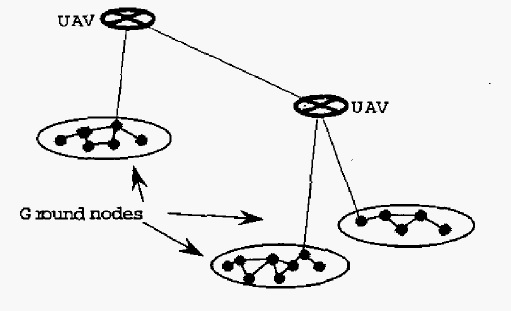
\includegraphics[scale=0.6]{scenario}
	\end{center}
	\caption{Backbone di UAVs per connettere gruppi isolati di utenti} \label{fig:scenario}
\end{figure}
%
Il posizionamento di ciascun drone, espresso in coordinate spaziali, è determinato tramite la risoluzione di un modello di programmazione lineare intera mista (Mixed Integer Linear Problem, o MILP). \\
L'elaborazione del modello è compiuta da una Ground Station, in posizione fissa e sempre raggiungibile da almeno un drone, che si occupa di mantenere uno stato interno della rete di UAV (la loro posizione, lo stato, la banda disponibile, i flussi di traffico attivi, etc.), risolvere il modello MILP quando richiesto (periodicamente o quando si verifica un evento esterno che richiede un ricalcolo delle posizioni, come l'arrivo di nuovi utenti o un drone che diventa offline) e inviare l'aggiornamento delle coordinate ai droni interessati (per esempio mediante flooding). \\
Risolvere un'istanza del modello MILP significa minimizzare il costo di deployment dei droni, ovvero calcolare le posizioni del minor numero possibile di UAV necessario a costruire una rete ad-hoc capace di interconnettere ogni utente, e soddisfare le sue richieste di traffico, espresse da una matrice di traffico data. \\

\section{Il grafo della rete} \label{sect:graforete}
L'area geografica può essere rappresentata bi-dimensionalmente come una griglia rettangolare discreta formata da $L$ x $H$ punti. \\
Chiamiamo $V$ l'insieme degli $n$ utenti posizionati staticamente sulla griglia, e $P$ l'insieme degli $L$ x $H$ punti facenti parte di essa. Definiamo inoltre l'insieme $V' = V \cup P$ come l'insieme dei punti e degli utenti. \\
Chiamiamo $P$ l'insieme dei punti potenziali della rete, ovvero l'insieme di tutti quei punti della griglia in cui può essere posizionato un drone. Assumiamo che, per motivi di sicurezza, non si possa posizionare un UAV in un punto in cui è già presente un utente. \\
La rete ad-hoc che si viene a creare può essere modellata come un grafo diretto, dove i nodi rappresentano i membri della rete, quindi sia gli utenti che i droni impiegati, mentre gli archi indicano le connessioni wireless tra i nodi. Ad ogni arco può venire assegnato un peso che indichi un generico tipo di costo trasmissivo (energetico o legato ai parametri della rete). Si può vedere un semplice esempio in \figurename\ \ref{fig:grid}, dove tre client (punti rossi) incapaci di comunicare direttamente (i cerchi rossi, rappresentanti il range di comunicazione, non si intersecano) vengono connessi tramite il posizionamento di un drone (punto blu). \\
%
\begin{figure}
	\begin{center}
		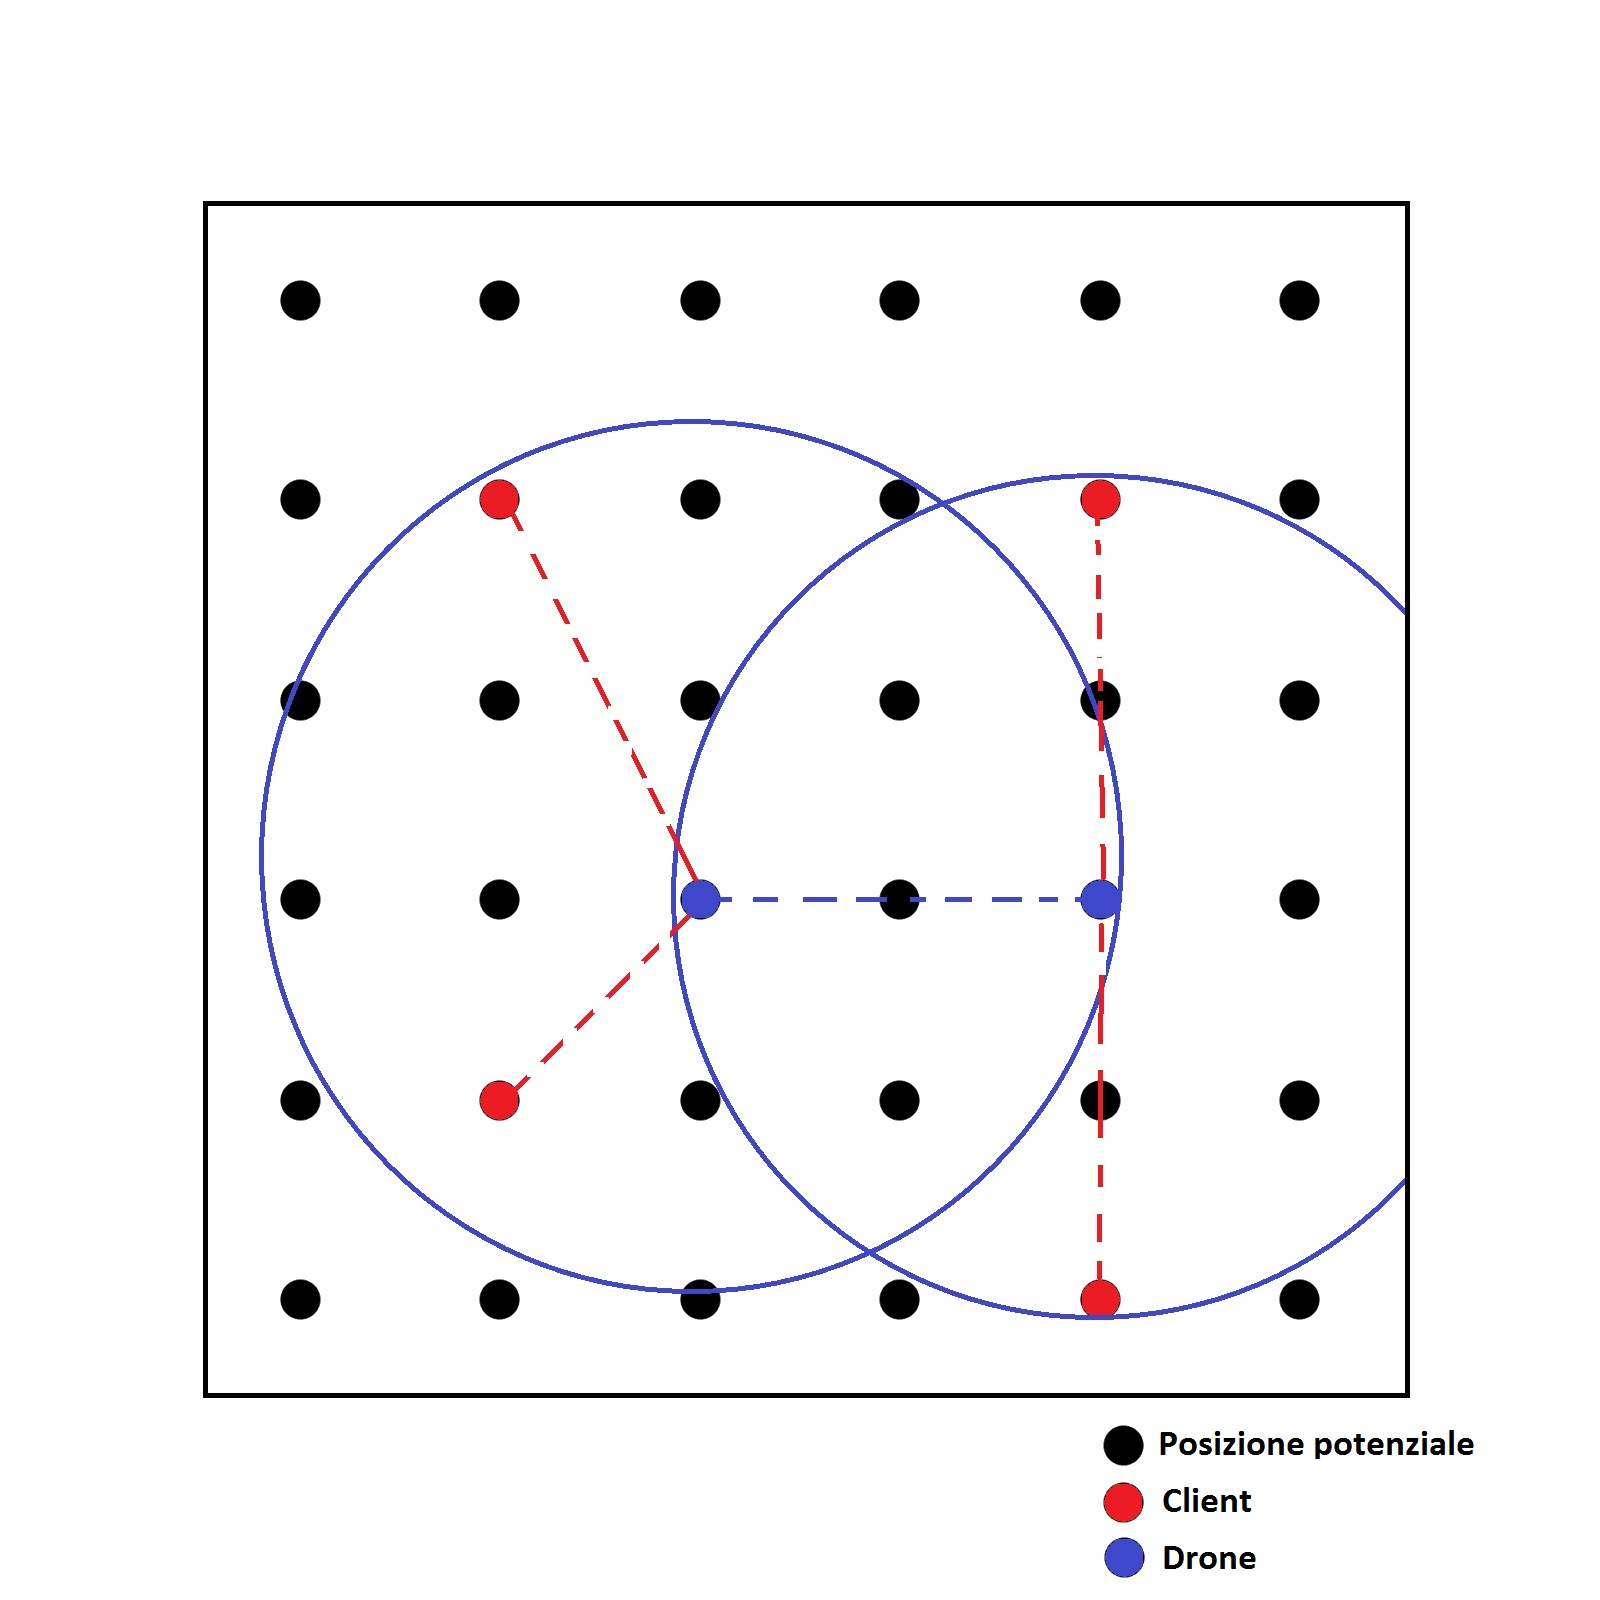
\includegraphics[scale=0.2]{grid}
	\end{center}
	\caption{Backbone di UAVs per connettere gruppi isolati di utenti} \label{fig:grid}
\end{figure}
%
Il modello risultante, che verrà introdotto nel capitolo \ref{chap:modello}, può essere descritto come l'ibridazione tra due tipici problemi di ottimizzazione, il Multi-Commodity Flow Problem e il Capacitated Hub Location Problem con allocazione multipla \cite{Alumur20081}. \\
La risoluzione del modello, infatti, può essere suddivisa logicamente in due passi sequenziali:
\begin{enumerate}  
	\item Individuare il numero minimo di droni necessari e la loro posizione ottimale sulla griglia; 
	\item Risolvere un problema di multi-commodity flow, dimensionando i flussi di traffico per ciascuna commodity, definite come coppie distinte di nodi sorgente-destinazione, per soddisfare le richieste di tutti i client.
\end{enumerate}
Un'istanza tipica del problema viene descritta con:
\begin{itemize}  
	\item Insieme $V$ degli $n$ utenti, ciascuno con coordinate $(x_i,y_i)$, con $i = 0,1,...,|V|$;
	\item Insieme $K$ delle commodities, con $|K| = n (n-1)$;
	\item Numero massimo di droni disponibili ($N_{UAV}$);
	\item Dimensione della griglia, in numero di punti;
	\item Costo di deployment di ciascun drone ($D_v$); 
	\item Matrice di traffico ($T_{sd}$, con $s,d \in V$);
	\item Matrice dei costi di trasmissione ($C_{ijk}$, con $i,j \in V', k \in K$);
\end{itemize}

\section{Assunzioni}
L'intrinseca complessità del problema trattato e la necessità primaria di mantenere la linearità del modello hanno richiesto, durante la fase di modellizzazione, di introdurre una serie di assunzioni e semplificazioni al problema originario, che verranno ora brevemente trattate. \\
Come descritto nella sezione \ref{sect:graforete}, modelleremo i droni, gli utenti e le loro posizioni come nodi fissi di un grafo posizionato all'interno di una griglia di punti. La staticità degli utenti è motivata dalla complessità di integrare, in maniera diretta, modelli che simulino il movimento casuale in un problema lineare \cite{Johnson1996, bai2004survey}. Si può però creare una simulazione "offline" di spostamento risolvendo iterativamente un'istanza con set di coordinate ogni volta diverse, ottenute applicando, in pre-elaborazione, modelli di movimento casuale agli utenti.\\
Nel modello non verranno introdotte le specifiche tecniche dei droni e non considereremo un modello realistico di volo: assumeremo solamente che tutti gli UAV siano tra loro identici, in fatto di performance e caratteristiche tecniche, e che siano in grado di muoversi autonomamente in linea retta da una posizione $(x,y,z)$ ad un'altra, senza collidere con eventuali ostacoli lungo il cammino. Questa scelta consente di mantenere questi aspetti al di fuori del modello MILP, delegandoli ai droni stessi (per esempio con funzionalità di guida autonoma) o alla ground station. \\
Assumeremo inoltre che l'area geografica in cui si trovano gli utenti sia pianeggiante e priva di ostacoli naturali, come alberi, monti o depressioni, o artificiali, come edifici o altre barriere (open field), simulando così un ambiente con condizioni ottimali per la trasmissione e un ridotto numero di sorgenti di interferenza che devono essere gestite dal modello. \\
Riguardo gli utenti, assumiamo che il traffico da loro generato sia una piccola percentuale della capacità complessiva di un nodo, così da poter trascurare gli effetti dell'interferenza da loro causata sui droni. \\
Come evidenziato nella sezione \ref{sect:autonomia}, attualmente uno dei principali limiti dei droni è dato dalla esigua autonomia di volo. 
In questo modello assumeremo che i droni siano energeticamente autosufficienti, tramite l'uso di pannelli solari ad alta efficienza \cite{alta} o impiegando un sistema automatizzato di stazioni di ricarica \cite{Song2014}, così da poter fornire un servizio continuo e persistente. 
Questa scelta rende impossibile il verificarsi di link failures, e il conseguente cambio di topologia, ma può essere simulato risolvendo nuovamente un'istanza con un numero ridotto di droni o vietandone il deployment in certi punti potenziali (No Flight Zones). \\
Dal punto di vista della rete, non considereremo alcun parametro di Quality of Service (QoS) \cite{6686488} e, per mantenere semplice la modellizzazione del grafo, assumeremo che i nodi possano comunicare in modalità full-duplex \cite{6262501}, in modo che sia l'arco diretto che quello inverso possano esistere contemporaneamente.  \\
Assumeremo inoltre che l'overhead causato dal traffico di controllo, come l'ACK signaling del protocollo TCP, i messaggi di routing o il flooding per diffondere informazioni tra i droni, sia di dimensione trascurabile. 
Consideriamo inoltre che tutti i devices Wi-Fi montati sui droni e posseduti dagli utenti siano identici in termini di bandwidth, potenza trasmessa (la massima permessa) e range massimo di trasmissione/ricezione (TX/RX) e che siano equipaggiati con antenne ideali isotropiche \cite{zennaro2004radio} che non subiscono interferenza elettromagnetica dagli apparati del drone. \\
Infine, per evitare l'introduzione di un secondo problema di ottimizzazione relativo all'assegnazione delle frequenze, assumiamo che tutti i nodi della rete condividano lo stesso canale wireless. 
Come conseguenza di ciò la trasmissione di ogni nodo causerà interferenza co-channel \cite{arokiamary2009cellular} a tutte le altre trasmittenti entro il suo range, con intensità dipendente dalle distanze reciproche.
 





